\documentclass[8pt,aspectratio=169]{beamer}
\usetheme{Madrid}
\usepackage{graphicx}
\usepackage{booktabs}
\usepackage{adjustbox}
\usepackage{multicol}
\usepackage{amsmath}
\usepackage{amssymb}
\usepackage{tikz}
\usepackage{hyperref}
\usepackage{algorithm}
\usepackage{algorithmic}
\usepackage{colortbl}
\usepackage{pgfplots}
\pgfplotsset{compat=1.18}

% TikZ libraries for comics, diagrams, stakeholder maps
\usetikzlibrary{arrows.meta,positioning,shapes.callouts,shapes.geometric,decorations.pathreplacing}

% Color definitions
\definecolor{mlblue}{RGB}{0,102,204}
\definecolor{mlpurple}{RGB}{51,51,178}
\definecolor{mllavender}{RGB}{173,173,224}
\definecolor{mllavender2}{RGB}{193,193,232}
\definecolor{mllavender3}{RGB}{204,204,235}
\definecolor{mllavender4}{RGB}{214,214,239}
\definecolor{mlorange}{RGB}{255, 127, 14}
\definecolor{mlgreen}{RGB}{44, 160, 44}
\definecolor{mlred}{RGB}{214, 39, 40}
\definecolor{mlgray}{RGB}{127, 127, 127}
\definecolor{lightgray}{RGB}{240, 240, 240}
\definecolor{midgray}{RGB}{180, 180, 180}

% NEW COLORS for mini-lecture
\definecolor{dfteal}{RGB}{0,128,128}
\definecolor{dfred}{RGB}{180,30,30}

% Backward compatibility
\colorlet{MLPurple}{mlpurple}
\colorlet{MLBlue}{mlblue}
\colorlet{MLOrange}{mlorange}
\colorlet{MLGreen}{mlgreen}
\colorlet{MLRed}{mlred}
\colorlet{MLLavender}{mllavender}
\colorlet{MLGray}{mlgray}

% Theme colors (exact Madrid settings)
\setbeamercolor{palette primary}{bg=mllavender3,fg=mlpurple}
\setbeamercolor{palette secondary}{bg=mllavender2,fg=mlpurple}
\setbeamercolor{palette tertiary}{bg=mllavender,fg=white}
\setbeamercolor{palette quaternary}{bg=mlpurple,fg=white}
\setbeamercolor{structure}{fg=mlpurple}
\setbeamercolor{section in toc}{fg=mlpurple}
\setbeamercolor{subsection in toc}{fg=mlblue}
\setbeamercolor{title}{fg=mlpurple}
\setbeamercolor{frametitle}{fg=mlpurple,bg=mllavender3}
\setbeamercolor{block title}{bg=mllavender2,fg=mlpurple}
\setbeamercolor{block body}{bg=mllavender4,fg=black}
\setbeamertemplate{navigation symbols}{}
\setbeamertemplate{itemize items}[circle]
\setbeamertemplate{enumerate items}[default]
\setbeamersize{text margin left=5mm,text margin right=5mm}

% Footer
\setbeamertemplate{footline}{
  \leavevmode%
  \hbox{%
    \begin{beamercolorbox}[wd=.333333\paperwidth,ht=2.25ex,dp=1ex,center]{author in head/foot}%
      \usebeamerfont{author in head/foot}Methods and Algorithms
    \end{beamercolorbox}%
    \begin{beamercolorbox}[wd=.333333\paperwidth,ht=2.25ex,dp=1ex,center]{title in head/foot}%
      \usebeamerfont{title in head/foot}MSc Data Science
    \end{beamercolorbox}%
    \begin{beamercolorbox}[wd=.333333\paperwidth,ht=2.25ex,dp=1ex,right]{date in head/foot}%
      \usebeamerfont{date in head/foot}\insertframenumber{} / \inserttotalframenumber\hspace*{2ex}
    \end{beamercolorbox}}%
  \vskip0pt%
}

\newcommand{\bottomnote}[1]{%
\vfill
\vspace{-2mm}
\textcolor{mllavender2}{\rule{\textwidth}{0.4pt}}
\vspace{1mm}
\footnotesize
\textbf{#1}
}

\newenvironment{compactlist}{%
  \begin{itemize}%
    \setlength{\itemsep}{2pt}%
    \setlength{\parskip}{0pt}%
    \setlength{\parsep}{0pt}%
}{%
  \end{itemize}%
}

\newcommand{\highlight}[1]{\textcolor{mlorange}{\textbf{#1}}}
\newcommand{\mathbold}[1]{\boldsymbol{#1}}

%-----------------------------------------------------------
\title{PCA \& t-SNE: A Visual Guide}
\subtitle{No Formulas, Just Pictures}
\author{Prof.\ Dr.\ J\"org Osterrieder}
\institute{Methods and Algorithms --- MSc Data Science}
\date{Spring 2026}
%-----------------------------------------------------------

\begin{document}

%=== Slide 1: Title Page ===
\begin{frame}[plain]
\titlepage
\end{frame}

%=== Slide 2: XKCD Opening ===
\begin{frame}{When You Have Too Many Dimensions}
\begin{columns}[T]
\begin{column}{0.55\textwidth}
\centering
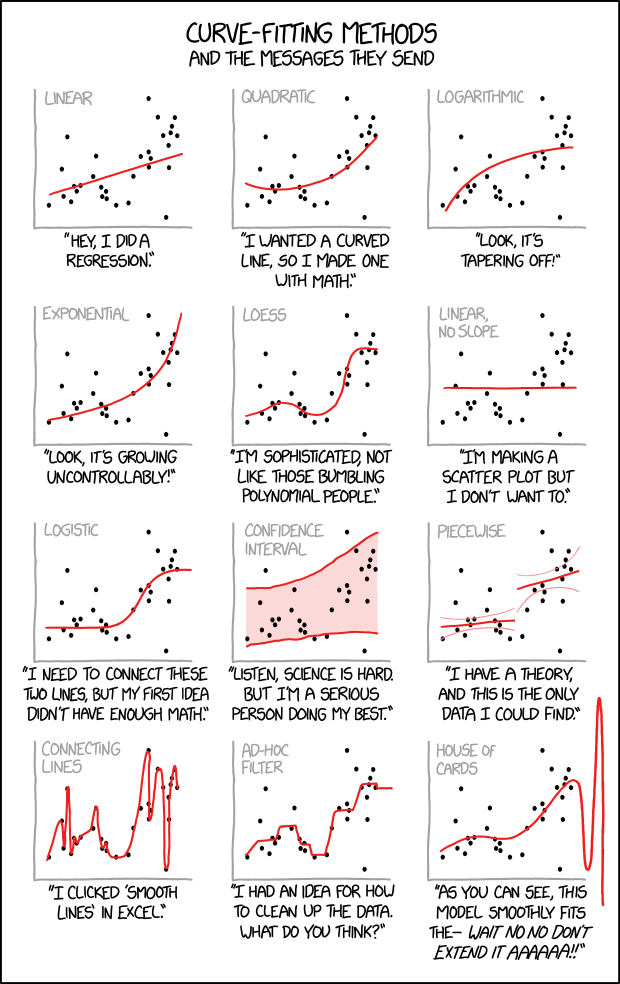
\includegraphics[height=0.55\textheight]{images/2048_curve_fitting.png}
\end{column}
\begin{column}{0.42\textwidth}
\vspace{8mm}
Your dataset has 50 columns.\\[4mm]
You can only plot 2 axes.\\[4mm]
\highlight{What do you do?}
\end{column}
\end{columns}
\bottomnote{XKCD \#2048 by Randall Munroe (CC BY-NC 2.5)}
\end{frame}

%=== Slide 3: Learning Objectives ===
\begin{frame}{What You Will Learn Today}
\begin{enumerate}
  \setlength{\itemsep}{6pt}
  \item Explain what PCA does --- without any formulas
  \item Describe when t-SNE beats PCA
  \item Choose the right method for a given dataset
\end{enumerate}
\bottomnote{No formulas in this lecture. Everything is explained with pictures and analogies.}
\end{frame}

%===========================================================
\section{The Problem}
%===========================================================

%=== Slide 4: TikZ Comic C1 --- Drowning in Dimensions ===
\begin{frame}{The Problem: Too Many Features!}
\centering
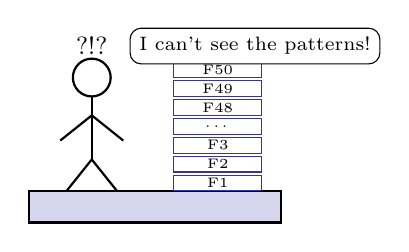
\begin{tikzpicture}[scale=0.8]
  % Desk
  \fill[mllavender4] (-1.5,-0.5) rectangle (2.5,0);
  \draw[thick] (-1.5,-0.5) rectangle (2.5,0);
  % Stack of papers
  \foreach \i/\lab in {0/F1,0.3/F2,0.6/F3,1.2/F48,1.5/F49,1.8/F50} {
    \fill[white] (0.8,\i) rectangle (2.2,\i+0.25);
    \draw[mlpurple] (0.8,\i) rectangle (2.2,\i+0.25);
    \node[font=\tiny] at (1.5,\i+0.125) {\lab};
  }
  % Dots between F3 and F48
  \fill[white] (0.8,0.9) rectangle (2.2,1.15);
  \draw[mlpurple] (0.8,0.9) rectangle (2.2,1.15);
  \node[font=\tiny] at (1.5,1.025) {\ldots};
  % Stick figure
  \draw[thick] (-0.5,1.8) circle (0.3); % head
  \draw[thick] (-0.5,1.5) -- (-0.5,0.5); % body
  \draw[thick] (-0.5,1.2) -- (-1.0,0.8); % left arm
  \draw[thick] (-0.5,1.2) -- (0.0,0.8); % right arm
  \draw[thick] (-0.5,0.5) -- (-0.9,0); % left leg
  \draw[thick] (-0.5,0.5) -- (-0.1,0); % right leg
  % Confused marks
  \node[font=\small] at (-0.5,2.3) {?!?};
  % Speech bubble
  \node[draw,rounded corners,fill=white,font=\scriptsize,anchor=west] at (0.1,2.3) {I can't see the patterns!};
\end{tikzpicture}

\vspace{3mm}
Imagine a bank tracking 50 risk metrics per portfolio. How do you visualize this?

\bottomnote{High-dimensional data is everywhere: genomics (20k genes), NLP (50k words), finance (hundreds of factors).}
\end{frame}

%=== Slide 5: CHART --- Before/After ===
\begin{frame}{Compression Works!}
\centering

\includegraphics[width=0.65\textwidth]{08_high_dim_before_after/chart.pdf}

\begin{compactlist}
  \item Each dot was originally described by 10 numbers (features)
  \item PCA compressed it to just 2 numbers
  \item The three clusters are still clearly visible
\end{compactlist}
\bottomnote{PCA found the 2 directions that preserve the most spread --- no human picked them.}
\end{frame}

%=== Slide 6: Why Not Just Pick 2? ===
\begin{frame}{Why Not Just Pick Two Features?}
\begin{columns}[T]
\begin{column}{0.47\textwidth}
\begin{block}{\textcolor{mlred}{Cherry-Picking}}
\begin{compactlist}
  \item Pick 2 out of 50 features
  \item Lose 48 features' information
  \item Which pair is best? Nobody knows
\end{compactlist}
\end{block}
\end{column}
\begin{column}{0.47\textwidth}
\begin{block}{\textcolor{mlgreen}{PCA Approach}}
\begin{compactlist}
  \item Blend ALL features into 2 new axes
  \item Automatic --- no guessing
  \item Keeps maximum information
\end{compactlist}
\end{block}
\end{column}
\end{columns}

\vspace{4mm}
\centering
\highlight{PCA does not discard features --- it blends them.}

\bottomnote{Selecting features = you choose. PCA = the data chooses the best blend.}
\end{frame}

%===========================================================
\section{PCA = Best Shadow}
%===========================================================

%=== Slide 7: TikZ Comic C2 --- The Shadow Analogy ===
\begin{frame}{PCA = Finding the Best Shadow}
\centering
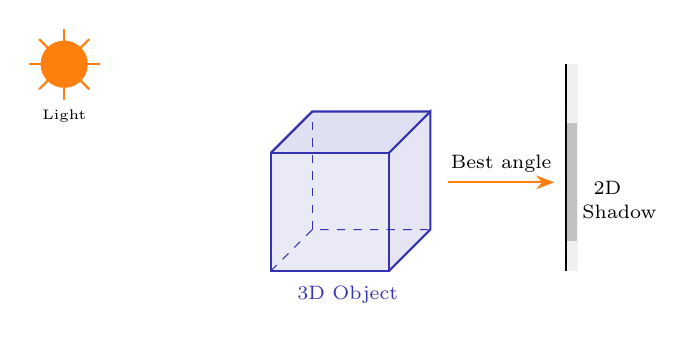
\begin{tikzpicture}[scale=0.75]
  % Sun
  \fill[mlorange] (-3.5,3.5) circle (0.4);
  \foreach \a in {0,45,...,315} {
    \draw[mlorange,thick] (-3.5,3.5) -- ++(\a:0.6);
  }
  \node[font=\tiny,below] at (-3.5,2.9) {Light};
  % 3D cube (manual)
  \coordinate (A) at (0,0);
  \coordinate (B) at (2,0);
  \coordinate (C) at (2,2);
  \coordinate (D) at (0,2);
  \coordinate (E) at (0.7,0.7);
  \coordinate (F) at (2.7,0.7);
  \coordinate (G) at (2.7,2.7);
  \coordinate (H) at (0.7,2.7);
  \fill[mllavender4,opacity=0.5] (A)--(B)--(C)--(D)--cycle;
  \fill[mllavender3,opacity=0.5] (B)--(F)--(G)--(C)--cycle;
  \fill[mllavender2,opacity=0.5] (D)--(C)--(G)--(H)--cycle;
  \draw[mlpurple,thick] (A)--(B)--(C)--(D)--cycle;
  \draw[mlpurple,thick] (B)--(F)--(G)--(C);
  \draw[mlpurple,thick] (D)--(H)--(G);
  \draw[mlpurple,dashed] (A)--(E)--(F);
  \draw[mlpurple,dashed] (E)--(H);
  \node[font=\scriptsize,mlpurple] at (1.3,-0.4) {3D Object};
  % Wall
  \fill[lightgray] (5,0) rectangle (5.2,3.5);
  \draw[thick] (5,0) -- (5,3.5);
  % Shadow on wall
  \fill[mlgray,opacity=0.6] (5,0.3) -- (5,2.8) -- (5,2.5) -- (5,0.5) -- cycle;
  \fill[mlgray,opacity=0.4] (5.01,0.5) rectangle (5.19,2.5);
  \node[font=\scriptsize] at (5.7,1.4) {2D};
  \node[font=\scriptsize] at (5.9,1.0) {Shadow};
  % Arrow
  \draw[-{Stealth},thick,mlorange] (3.0,1.5) -- (4.8,1.5);
  \node[font=\scriptsize,above] at (3.9,1.5) {Best angle};
\end{tikzpicture}

\vspace{3mm}
PCA finds the angle that makes the shadow show the most detail.

\bottomnote{PCA is literally a projection: it casts your high-dimensional data onto a lower-dimensional ``wall.''}
\end{frame}

%=== Slide 8: CHART --- Principal Components ===
\begin{frame}{PCA Finds the Best Directions}
\centering

\includegraphics[width=0.55\textwidth]{02_principal_components/chart.pdf}
\vspace{-1mm}
\begin{compactlist}
  \item The first arrow (PC1) points along the main cloud --- maximum spread
  \item The second arrow (PC2) is perpendicular --- remaining spread
  \item Together they form new coordinate axes
\end{compactlist}
\bottomnote{PCA is a rotation: it views your data from the angle that shows the most structure.}
\end{frame}

%=== Slide 9: Three Steps of PCA (TikZ flowchart) ===
\begin{frame}{PCA in Three Steps}
\centering
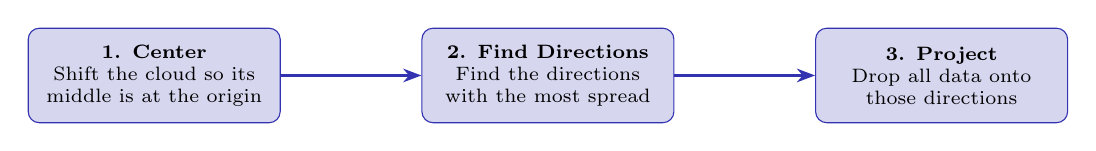
\begin{tikzpicture}[
  box/.style={draw=mlpurple, fill=mllavender4, rounded corners=4pt,
              minimum width=3.2cm, minimum height=1.2cm, align=center,
              font=\scriptsize},
  arr/.style={-{Stealth}, thick, mlpurple}
]
  \node[box] (s1) at (0,0) {\textbf{1. Center}\\Shift the cloud so its\\middle is at the origin};
  \node[box] (s2) at (5,0) {\textbf{2. Find Directions}\\Find the directions\\with the most spread};
  \node[box] (s3) at (10,0) {\textbf{3. Project}\\Drop all data onto\\those directions};
  \draw[arr] (s1) -- (s2);
  \draw[arr] (s2) -- (s3);
\end{tikzpicture}

\vspace{5mm}
\highlight{That's the entire algorithm. Three steps.}

\bottomnote{Step 2 uses eigenvalues internally, but you never need to compute them by hand --- sklearn does it.}
\end{frame}

%=== Slide 10: CHART --- Scree Plot ===
\begin{frame}{How Many Components Do We Keep?}
\centering

\includegraphics[width=0.60\textwidth]{01_scree_plot/chart.pdf}

\begin{compactlist}
  \item Bars = variance captured by each component (first few are tall)
  \item Line = cumulative total (crosses 80\% quickly)
  \item Stop at the ``elbow'' --- where adding more barely helps
\end{compactlist}
\bottomnote{Named after geological ``scree'' (cliff rubble). Stop where the cliff flattens into rubble.}
\end{frame}

%=== Slide 11: CHART --- PCA Clusters ===
\begin{frame}{PCA Separates Some Clusters\ldots}
\centering

\includegraphics[width=0.60\textwidth]{06b_pca_cluster_projection/chart.pdf}

\begin{compactlist}
  \item Each color is a different group
  \item PCA separates some groups well
  \item But overlapping groups stay mixed --- PCA is linear
\end{compactlist}
\bottomnote{PCA works great when clusters are separated by straight lines. But what if the data curves?}
\end{frame}

%=== Slide 12: Transition --- Limits of Straight Lines ===
\begin{frame}{The Limit of Straight Lines}
\centering
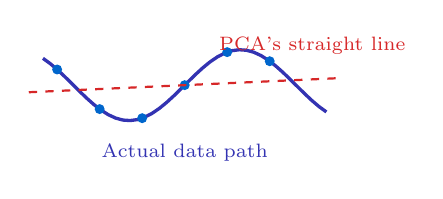
\begin{tikzpicture}[scale=0.9]
  % Curved data
  \draw[mlpurple, very thick, domain=-2:2, samples=40] plot (\x, {0.5*sin(deg(\x*2))});
  \foreach \x in {-1.8,-1.2,...,1.8} {
    \fill[mlblue] (\x, {0.5*sin(deg(\x*2))}) circle (2pt);
  }
  % Straight line through it
  \draw[mlred, thick, dashed] (-2.2,-0.1) -- (2.2,0.1);
  \node[font=\scriptsize, mlred, above] at (1.8,0.3) {PCA's straight line};
  \node[font=\scriptsize, mlpurple, below] at (0,-0.7) {Actual data path};
\end{tikzpicture}

\vspace{3mm}
\begin{compactlist}
  \item PCA uses straight lines (linear) --- great for flat data
  \item But real data often curves --- we need something smarter\ldots
\end{compactlist}

\bottomnote{When data lies on a curved surface, PCA cuts through it instead of following the curve.}
\end{frame}

%===========================================================
\section{t-SNE = Keep Neighbors Close}
%===========================================================

%=== Slide 13: TikZ Comic C3 --- The Neighborhood Rule ===
\begin{frame}{t-SNE: Keep Your Neighbors Close}
\centering
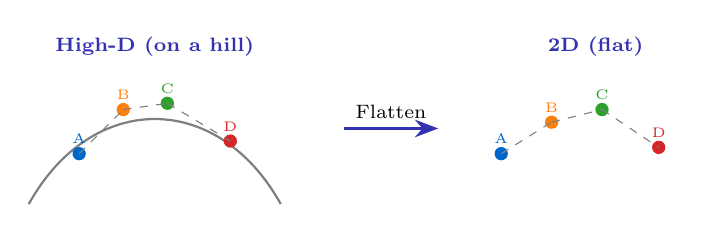
\begin{tikzpicture}[scale=0.8]
  % Left: curved surface with dots
  \node[font=\scriptsize\bfseries,mlpurple] at (-3,2.5) {High-D (on a hill)};
  \draw[mlgray, thick] (-5,0) .. controls (-4,1.8) and (-2,1.8) .. (-1,0);
  \fill[mlblue] (-4.2,0.8) circle (3pt) node[above,font=\tiny] {A};
  \fill[mlorange] (-3.5,1.5) circle (3pt) node[above,font=\tiny] {B};
  \fill[mlgreen] (-2.8,1.6) circle (3pt) node[above,font=\tiny] {C};
  \fill[mlred] (-1.8,1.0) circle (3pt) node[above,font=\tiny] {D};
  \draw[dashed,mlgray] (-4.2,0.8) -- (-3.5,1.5);
  \draw[dashed,mlgray] (-3.5,1.5) -- (-2.8,1.6);
  \draw[dashed,mlgray] (-2.8,1.6) -- (-1.8,1.0);
  % Arrow
  \draw[-{Stealth},very thick,mlpurple] (0,1.2) -- (1.5,1.2);
  \node[font=\scriptsize,above] at (0.75,1.2) {Flatten};
  % Right: flat with same neighbor structure
  \node[font=\scriptsize\bfseries,mlpurple] at (4,2.5) {2D (flat)};
  \fill[mlblue] (2.5,0.8) circle (3pt) node[above,font=\tiny] {A};
  \fill[mlorange] (3.3,1.3) circle (3pt) node[above,font=\tiny] {B};
  \fill[mlgreen] (4.1,1.5) circle (3pt) node[above,font=\tiny] {C};
  \fill[mlred] (5.0,0.9) circle (3pt) node[above,font=\tiny] {D};
  \draw[dashed,mlgray] (2.5,0.8) -- (3.3,1.3);
  \draw[dashed,mlgray] (3.3,1.3) -- (4.1,1.5);
  \draw[dashed,mlgray] (4.1,1.5) -- (5.0,0.9);
\end{tikzpicture}

\vspace{3mm}
t-SNE flattens the data while keeping nearby points nearby.

\bottomnote{t-SNE = t-distributed Stochastic Neighbor Embedding. The key idea: preserve local neighborhoods.}
\end{frame}

%=== Slide 14: CHART --- PCA Swiss Roll FAIL ===
\begin{frame}{PCA Fails on Curves: The Swiss Roll}
\centering

\includegraphics[width=0.65\textwidth]{05a_pca_swiss_roll/chart.pdf}

\begin{compactlist}
  \item The data spirals in 3D like a rolled carpet
  \item PCA smashes it flat --- distant points end up next to each other
\end{compactlist}
\bottomnote{PCA projects onto a plane, collapsing the spiral and mixing distant points.}
\end{frame}

%=== Slide 15: CHART --- t-SNE Swiss Roll WIN ===
\begin{frame}{t-SNE Unrolls the Carpet!}
\centering

\includegraphics[width=0.65\textwidth]{05b_tsne_swiss_roll/chart.pdf}

\begin{compactlist}
  \item t-SNE preserves local distances along the spiral
  \item Points that were neighbors on the roll stay neighbors in 2D
\end{compactlist}
\bottomnote{t-SNE successfully ``unrolls'' the manifold by preserving local neighbourhood structure.}
\end{frame}

%=== Slide 16: t-SNE in Plain English ===
\begin{frame}{How t-SNE Works (No Math)}
\begin{enumerate}
  \setlength{\itemsep}{3pt}
  \item \textbf{Measure neighborhoods} --- for each point, find its nearest neighbors
    \hfill
    
\begin{tikzpicture}[baseline=-2pt,scale=0.4]
      \fill[mlblue] (0,0) circle (3pt);
      \draw[mlgray,dashed] (0,0) circle (0.6);
      \fill[mlgray] (0.4,0.3) circle (2pt);
      \fill[mlgray] (-0.3,0.4) circle (2pt);
    \end{tikzpicture}
  \item \textbf{Scatter randomly} --- place all points on a 2D canvas at random
    \hfill
    \begin{tikzpicture}[baseline=-2pt,scale=0.4]
      \fill[mlblue] (0.1,0.3) circle (2pt);
      \fill[mlorange] (0.6,-0.1) circle (2pt);
      \fill[mlgreen] (-0.3,-0.2) circle (2pt);
      \fill[mlred] (0.4,0.5) circle (2pt);
    \end{tikzpicture}
  \item \textbf{Nudge until right} --- move points until 2D neighborhoods match the originals
    \hfill
    \begin{tikzpicture}[baseline=-2pt,scale=0.4]
      \fill[mlblue] (0,0) circle (2pt);
      \fill[mlorange] (0.25,0.15) circle (2pt);
      \fill[mlgreen] (-0.15,0.2) circle (2pt);
      \fill[mlred] (0.5,-0.05) circle (2pt);
    \end{tikzpicture}
\end{enumerate}

\vspace{3mm}
\begin{block}{Intuition}
Think of it as a spring system --- connected points pull each other close.
\end{block}

\bottomnote{t-SNE iterates hundreds of times, adjusting positions until the layout stabilizes.}
\end{frame}

%=== Slide 17: CHART --- t-SNE Clusters ===
\begin{frame}{t-SNE: Much Better Cluster Separation!}
\centering

\includegraphics[width=0.60\textwidth]{06c_tsne_cluster_projection/chart.pdf}

\begin{compactlist}
  \item Compare this with the PCA version (slide 11)
  \item t-SNE pulls apart clusters that PCA left overlapping
  \item The groups are now clearly separated
\end{compactlist}
\bottomnote{t-SNE excels at revealing clusters. But warning: inter-cluster distances are NOT meaningful.}
\end{frame}

%=== Slide 18: t-SNE Gotchas ===
\begin{frame}{Three Things to Watch Out For}
\begin{enumerate}
  \setlength{\itemsep}{5pt}
  \item \textcolor{mlred}{\textbf{!}} \textbf{Distances between clusters mean nothing}\\
    Only within-cluster structure is reliable
  \item \textcolor{mlred}{\textbf{!}} \textbf{Run it multiple times}\\
    Different random seeds give different layouts
  \item \textcolor{mlred}{\textbf{!}} \textbf{Slow on big data}\\
    Use PCA first to reduce to 50 dimensions, then run t-SNE
\end{enumerate}
\bottomnote{t-SNE is for visualization only. Never use t-SNE coordinates as input features for a classifier.}
\end{frame}

%===========================================================
\section{When to Use What}
%===========================================================

%=== Slide 19: PCA vs t-SNE Side-by-Side ===
\begin{frame}{PCA vs t-SNE: Quick Comparison}
\centering
\begin{tabular}{lll}
\toprule
\textbf{Aspect} & \textbf{PCA} & \textbf{t-SNE} \\
\midrule
Type & Linear & Non-linear \\
Preserves & Global structure & Local neighborhoods \\
Speed & Fast (seconds) & Slow (minutes) \\
Output & New features for ML & 2D plot only \\
Deterministic & Yes & No (random seed) \\
\bottomrule
\end{tabular}

\vspace{5mm}
\highlight{They are complementary tools, not competitors.}\\
Use PCA to preprocess, t-SNE to visualize.

\bottomnote{In practice, run PCA to 50 dims first, then apply t-SNE for visualization.}
\end{frame}

%=== Slide 20: CHART --- Decision Flowchart ===
\begin{frame}{Which Method Should I Use?}
\centering

\includegraphics[width=0.60\textwidth]{07_decision_flowchart/chart.pdf}
\vspace{-1mm}
\begin{compactlist}
  \item Start at the top and follow the arrows
  \item In practice, try both and compare
\end{compactlist}
\bottomnote{When in doubt: run PCA first (fast, interpretable), then t-SNE for visualization.}
\end{frame}

%=== Slide 21: Finance Teaser ===
\begin{frame}{Why Bankers Love PCA}
\begin{columns}[T]
\begin{column}{0.55\textwidth}
\begin{compactlist}
  \item Bond markets track dozens of interest rates
  \item PCA reveals just 3 hidden factors:\\Level, Slope, Curvature
  \item These 3 factors explain over 98\% of all bond price movements
\end{compactlist}
\end{column}
\begin{column}{0.40\textwidth}
\centering
\vspace{2mm}
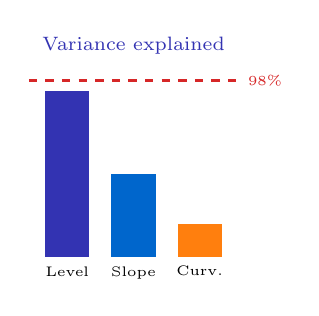
\begin{tikzpicture}[scale=0.7]
  \fill[mlpurple] (0,0) rectangle (0.8,3.0);
  \fill[mlblue]   (1.2,0) rectangle (2.0,1.5);
  \fill[mlorange] (2.4,0) rectangle (3.2,0.6);
  \node[font=\tiny,below] at (0.4,0) {Level};
  \node[font=\tiny,below] at (1.6,0) {Slope};
  \node[font=\tiny,below] at (2.8,0) {Curv.};
  \draw[mlred,thick,dashed] (-0.3,3.2) -- (3.5,3.2);
  \node[font=\tiny,mlred,right] at (3.5,3.2) {98\%};
  \node[font=\scriptsize,mlpurple,above] at (1.6,3.5) {Variance explained};
\end{tikzpicture}
\end{column}
\end{columns}
\bottomnote{Litterman \& Scheinkman (1991): 3 PCA factors explain $>$98\% of US Treasury yield curve movements.}
\end{frame}

%=== Slide 22: The 5-Line Python Recipe ===
\begin{frame}{Try It Yourself: 5 Lines of Python}
\begin{columns}[T]
\begin{column}{0.47\textwidth}
\begin{block}{PCA}
\ttfamily\scriptsize
from sklearn.decomposition import PCA\\
pca = PCA(n\_components=2)\\
X\_reduced = pca.fit\_transform(X)
\end{block}
\end{column}
\begin{column}{0.47\textwidth}
\begin{block}{t-SNE}
\ttfamily\scriptsize
from sklearn.manifold import TSNE\\
tsne = TSNE(n\_components=2)\\
X\_embedded = tsne.fit\_transform(X)
\end{block}
\end{column}
\end{columns}

\vspace{5mm}
\centering
\highlight{That's it. Three lines each.} sklearn does the heavy lifting.

\bottomnote{Always scale your data first: \texttt{StandardScaler().fit\_transform(X)} before PCA.}
\end{frame}

%===========================================================
\section{Closing}
%===========================================================

%=== Slide 23: TikZ Comic C4 --- Now I See! ===
\begin{frame}{From Chaos to Clarity}
\centering
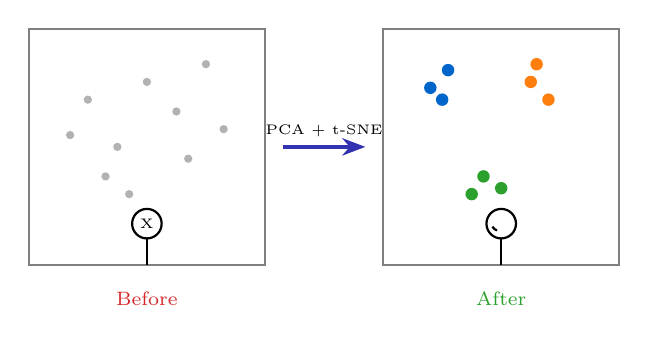
\begin{tikzpicture}[scale=0.75]
  % Left panel: confused
  \draw[mlgray,thick] (-5.5,-1) rectangle (-1.5,3);
  % Messy dots
  \foreach \x/\y in {-4.8/1.2,-4.2/0.5,-3.5/2.1,-2.8/0.8,-3.0/1.6,-4.5/1.8,-2.2/1.3,-3.8/0.2,-2.5/2.4,-4.0/1.0} {
    \fill[mlgray!60] (\x,\y) circle (2pt);
  }
  % Stick figure confused
  \draw[thick] (-3.5,-0.3) circle (0.25);
  \node[font=\tiny] at (-3.5,-0.3) {X};
  \draw[thick] (-3.5,-0.55) -- (-3.5,-1.0);
  \node[font=\scriptsize,below] at (-3.5,-1.3) {\textcolor{mlred}{Before}};
  %
  % Arrow
  \draw[-{Stealth},very thick,mlpurple] (-1.2,1.0) -- (0.2,1.0);
  \node[font=\tiny,above] at (-0.5,1.0) {PCA + t-SNE};
  %
  % Right panel: clear
  \draw[mlgray,thick] (0.5,-1) rectangle (4.5,3);
  % Clean clusters
  \fill[mlblue] (1.3,2.0) circle (3pt);
  \fill[mlblue] (1.6,2.3) circle (3pt);
  \fill[mlblue] (1.5,1.8) circle (3pt);
  \fill[mlorange] (3.0,2.1) circle (3pt);
  \fill[mlorange] (3.3,1.8) circle (3pt);
  \fill[mlorange] (3.1,2.4) circle (3pt);
  \fill[mlgreen] (2.2,0.5) circle (3pt);
  \fill[mlgreen] (2.5,0.3) circle (3pt);
  \fill[mlgreen] (2.0,0.2) circle (3pt);
  % Stick figure happy
  \draw[thick] (2.5,-0.3) circle (0.25);
  \draw[thick] (2.35,-0.35) arc (210:250:0.15); % smile
  \draw[thick] (2.5,-0.55) -- (2.5,-1.0);
  \node[font=\scriptsize,below] at (2.5,-1.3) {\textcolor{mlgreen}{After}};
\end{tikzpicture}

\bottomnote{Dimensionality reduction turns overwhelming data into actionable visualizations.}
\end{frame}

%=== Slide 24: Key Takeaways ===
\begin{frame}{Five Things to Remember}
\begin{enumerate}
  \setlength{\itemsep}{4pt}
  \item High-dimensional data is hard to see --- PCA and t-SNE make it visible
  \item PCA blends features into new axes that capture maximum spread
  \item t-SNE preserves neighborhoods --- great for finding clusters
  \item PCA is fast and gives you new features; t-SNE is slow but reveals hidden groups
  \item In finance, 3 PCA factors explain nearly all bond market movement
\end{enumerate}
\bottomnote{PCA for preprocessing and speed. t-SNE for visualization and cluster discovery. Use both.}
\end{frame}

%=== Slide 25: XKCD Closing ===
\begin{frame}{Go Find the Signal in the Noise}
\centering

\includegraphics[height=0.55\textheight]{images/2400_statistics.png}
\bottomnote{XKCD \#2400 by Randall Munroe (CC BY-NC 2.5). Next: try the Jupyter notebook with real financial data!}
\end{frame}

\end{document}
